\documentclass[tikz]{standalone}
\usepackage{amsmath, xcolor}
\boldmath

\colorlet{Green}{green!70!black}
\colorlet{Magenta}{magenta!90!black}
\colorlet{Yellow}{yellow!75!black}

\newcommand\quark[2]{\color{#1}$#2$}
\newcommand\anti[2]{\color{#1}$\bar{#2}$}
\newcommand\R{\quark{red}}
\newcommand\G{\quark{Green}}
\newcommand\B{\quark{blue}}
\newcommand\C{\anti{cyan}}
\newcommand\M{\anti{Magenta}}
\newcommand\Y{\anti{Yellow}}
\newcommand\K{\quark{black}}

\begin{document}
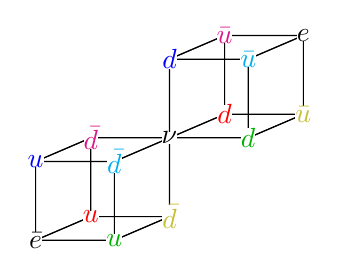
\begin{tikzpicture}[
  z={(0cm,1cm)},
  y={(1cm,0cm)},
  x={(7mm,3mm)},
  inner sep=0mm,
  every node/.style={fill=white}
  ]
\foreach \x/\y/\z/\i in {
  -1/-1/-1/1, 0/0/0/1, 0/0/0/-1, 1/1/1/-1}{
  \draw (\x,\y,\z) --++(right:\i) --++(up:\i)
  --++(left:\i) --++(down:\i);
  \draw (\x,\y,\z) --++(right:\i) --++(0,0,\i)
  --++(left:\i) --++(0,0,-\i);
  \draw (\x,\y,\z) --++(0,0,\i) --++(up:\i)
  --++(0,0,-\i) --++(down:\i);}
\draw
  (0,0,0) node {\K\nu}
  (1,0,0) node (red) {\R d}
  (0,1,0) node (green) {\G d}
  (0,0,1) node (blue) {\B d}
  (-1,0,0) node {\C d}
  (0,-1,0) node {\M d}
  (0,0,-1) node {\Y d}
  (-1,-1,-1) node {\K{\bar e}}
  (0,-1,-1) node {\R u}
  (-1,0,-1) node {\G u}
  (-1,-1,0) node {\B u}
  (1,1,1) node {\K e}
  (0,1,1) node {\C u}
  (1,0,1) node {\M u}
  (1,1,0) node {\Y u}
  ;
\end{tikzpicture}
\end{document}